\documentclass{ximera}

\title{Calculus on Curves: Velocities and Derivatives}
\author{Zack Reed}

\begin{document}
\begin{abstract}
In this activity we explore the concept of derivatives and velocity vectors for curves defined by vector functions. 
\end{abstract}
\maketitle

\section*{Tangent Vectors and Velocity}

\subsection*{From Single-Variable to Vector Derivatives}

Computing derivatives of vector functions is straightforward: we differentiate each component function and make a vector out of the results.

Despite this computational simplicity, it is important to spend some time understanding what the derivative represents. And how we might visualize it.

\begin{center}
\youtube{RZI8DKYpcIo}
\end{center}

\begin{problem}
In single-variable calculus, the derivative let you treat the function as if it were a line in small neighborhoods.

In the spirit of working with vectors, the following applet visualizes not just the tangent approximation, but uses a vector to represent the direction and the rate of change given by the derivative.

\begin{expandable}{stuff}{GeoGebra Instructions}
    Alter the ``X='' slider to see the tangent line shift along the curve. Notice the approximating horizontal and vertical components represented by $dx$ and $df$.
\end{expandable}

\begin{center}
\geogebra{gyh4uhzy}{786}{584}
\end{center}

Which of the following vectors represents the derivative at $x=\frac{\pi}{2}$ (appproximately $1.57$)?
\begin{multipleChoice}
    \choice{$[.55, 1]$}
    \choice[correct]{$[1, -.55]$}
    \choice{$[.55, -1]$}
    \choice{$[-1, .55]$}
\end{multipleChoice}
\begin{feedback}
The derivative represents the rate of change, which can be thought of as how much to change vertically for a unit change horizontally. This is not too different from how to think about a vector. 

If we consider a unit change in $x$ (i.e. $dx=1$), then the vector $[dx, df]$ represents the derivative.
\end{feedback}
\end{problem}

Motion is a very useful context to keep in mind when performing calculus on curves. The intuition of a ``velocity'' determining the direction and speed of motion is a very helpful way to conceptualize local linearity for both derivative and integral calculations.

\subsection*{Velocity Vectors One Component at a Time}

Let's return to the helix $\vec{r}(t) = [ \cos(t), \sin(t), t ]$. We compute the derivatives of each component function and put them together to make a velocity vector.

\begin{center}
\youtube{DwRRANqjIg0}
\end{center}

\begin{problem}

\begin{expandable}{stuff}{GeoGebra Instructions}
    Alter the ``t='' slider to view the velocity vector at different points. Click and drag to rotate your view. Notice how the vector is always tangent to the curve.
\end{expandable}

\begin{center}
\geogebra{zr86834p}{730}{487}
\end{center}

Complete the following statements by typing in the correct functions.

The derivative of the $x$-component $\cos(t)$ is: $\answer{-\sin(t)}$.

The derivative of the $y$-component $\sin(t)$ is: $\answer{\cos(t)}$.

The derivative of the $z$-component $t$ is: $\answer{1}$.

The three derivatives together form the velocity vector: $\vec{v}(t) = [\answer{-\sin(t)}, \answer{\cos(t)}, \answer{1}]$.

In the applet, the velocity vector is shown \wordChoice{\choice{at the origin}\choice[correct]{at the point on the curve}}\  corresponding to the current value of $t$ and represents (select all appropriate statements) \begin{selectAll}
    \choice{the position of the next particle location after a little time $dt$ has passed.}
    \choice[correct]{the direction towards which the curve is moving after time $t$.}
    \choice{the acceleration of the particle at time $t$.}
    \choice[correct]{the direction and speed that a particle will move as time changes by $dt$.}
\end{selectAll}
\end{problem}

\begin{definition}
For a vector function $\vec{r}(t) = \left[x(t), y(t), z(t) \right]$, the \textbf{velocity vector} (or \textbf{tangent vector}) is:
$$\vec{v}(t) = \vec{r}'(t) = \left[ \frac{dx}{dt}, \frac{dy}{dt}, \frac{dz}{dt} \right] = \left[ x'(t), y'(t), z'(t) \right]$$

This vector is tangent to the curve and points in the direction of motion.
\end{definition}

\begin{problem}
Let's compute some velocity vectors. If $\vec{r}(t) = [ t^2, 3t, 2t^3 ]$, find $\vec{v}(t)$.

$\vec{v}(t) = [ \answer{2t}, \answer{3}, \answer{6t^2} ]$

At $t=1$: $\vec{v}(1) = [ \answer{2}, \answer{3}, \answer{6} ]$

At $t=2$: $\vec{v}(2) = [ \answer{4}, \answer{3}, \answer{24} ]$

\begin{feedback}
Remember the power rule when taking derivatives! Also evaluate each component function at the specified $t$ values when wanting particular velocity vectors.
\end{feedback}
\end{problem}

\begin{problem}
After exploring the helix applet, select all true statements about velocity vectors:
\begin{selectAll}
    \choice[correct]{The velocity vector is always tangent to the curve}
    \choice[correct]{The velocity vector's direction can change as the particle moves}
    \choice{The velocity vector is always the same length}
    \choice[correct]{The velocity vector points in the direction of motion (that is, the direction representing positive time)}
\end{selectAll}
\end{problem}

\section*{Same Curve Different Speeds - Torty and Harry}

We can carry the velocity analogy even further. 

If you consider a vector curve as a path, you can run along a path at various speeds without changing the path. Likewise, you can have different velocities along the same curve without changing fundamental features of the curves.

To explore this, let's return to the race between Torty and Harry from Calculus 1! 

After Torty's victory, Harry is attempting to use a hilly terrain to his advantage.

\begin{center}
    \youtube{1j-cbvNrO0w}
\end{center}

Harry has become quite adjusted to racing along inclines and declines. His path in the provided GeoGebra applet is defined by the curve $h(t)=[ \cos(t), \sin(t), \cos(t)\sin^2(t)]$, for which two laps around the course takes $4 \pi$ seconds.

In their rematch, Torty is less adjusted to running along hilly regions and tires after bursts of speed. His path in the provided GeoGebra applet is defined by the curve $\tau (t)=[ \cos(t+\sin(t)), \sin(t+\sin(t)), \cos(t+\sin(t))\sin^2(t+\sin(t))]$.

\begin{problem}
    Before exploring the applet, answer the following question:

    Based on the definition of the two curves, which of the following statements is true?

    \begin{multipleChoice}
        \choice{They follow different paths and move at different speeds}
        \choice{They follow different paths but move at the same speed}
        \choice{They follow the same path and move at the same speed}
        \choice[correct]{They follow the same path but move at different speeds}
    \end{multipleChoice}

    \begin{feedback}
        Think about the outputs of the functions $h(t)$ and $\tau(t)$ and the positions they represent.

        Then, compare the following graphs of the parameterizations $t$ and $t+\sin(t)$ to understand how the speeds differ.

        %make a tikz plot of t vs t+sin(t)
        \begin{center}
        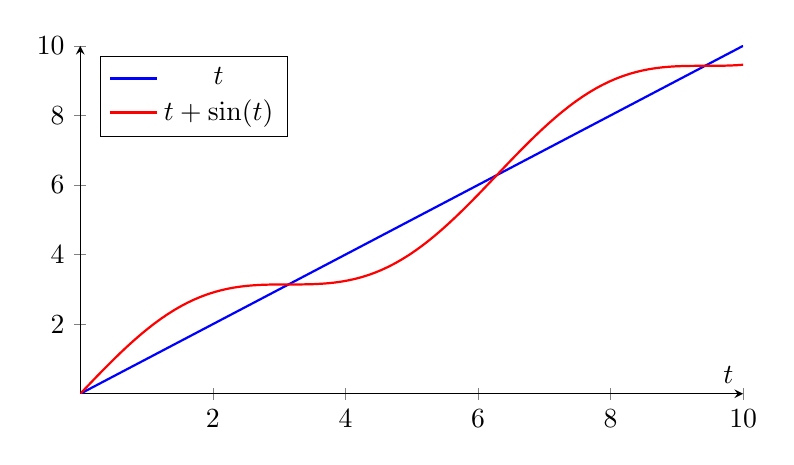
\begin{tikzpicture}
            \begin{axis}[
                axis lines = middle,
                xlabel = $t$,
                domain=0:10,
                samples=100,
                width=10cm,
                height=6cm,
                legend pos=north west,
            ]
            \addplot [blue, thick] {x};
            \addlegendentry{$t$}
            \addplot [red, thick] {x + sin(deg(x))};
            \addlegendentry{$t + \sin(t)$}
            \end{axis}
        \end{tikzpicture}
        \end{center}
    \end{feedback}
\end{problem}

Now let's take a look at how their race unfolds.

\begin{expandable}{stuff}{GeoGebra Instructions}
    You may alter the ``t='' slider to view Torty and Harry's positions, velocities, and accelerations at any time during the race. You may also use the ``Show Torty's Curve'' and ``Show Harry's Curve'' checkboxes to view either of the racer's curve in isolation.
\end{expandable}

\begin{center}
\geogebra{yzxdk5uw}{844}{629}
\end{center}

\begin{problem}
    As depicted in the applet, both racers follow \wordChoice{\choice{different}\choice[correct]{the same}} path(s). They also move along the path(s) at \wordChoice{\choice[correct]{different}\choice{the same}} speed(s).

    \begin{feedback}
        The only difference between the racers' positions is the parameterization of time. Altering the passing of time alters the speed at which the positions along the path are met, but does not alter the path itself (as long as time only moves forward).
    \end{feedback}
\end{problem}

\begin{remark}
    The key difference between the two racers is the parameterization of time. Harry's position at time $t$ is given by $h(t)$, while Torty's position at time $t$ is given by $\tau(t)=h(t+\sin(t))$. The additional $\sin(t)$ term in Torty's parameterization causes him to speed up and slow down periodically, affecting his overall speed along the same path.
\end{remark}

\subsection*{Speed and Velocity}

Now let's understand the difference between the racers' velocities. 

\begin{problem}
    Remember that the velocity vector is found by taking the derivative of each component function to form a new vector function. 
    
    \begin{expandable}{stuff}{Formula Answer Boxes}
        These answers require you to put in mathematical expressions like $\sin(t)$, $\cos(t)$, $sin^2(t)$, etc. Type them in as you would in a math editor, do not use latex formatting or backslashes. For example, type ``sin(t)'' for $\sin(t)$ and ``sin\^2(t)'' for $\sin^2(t)$.
    \end{expandable}

    The velocity vector of Harry at time $t$ is given by $h'(t)=\frac{d}{dt}\left[ \answer{\cos(t)}, \answer{\sin(t)}, \answer{\cos(t) \sin(t)^2}\right]$.
    
    Taking each of these derivatives, we get:

    \[h'(t)=[ \answer{-\sin(t)}, \answer{\cos(t)}, \answer[given]{-\sin^3(t) + 2\cos^2(t) \sin(t)}]\]
    \begin{feedback}
        Don't forget that the variable is $t$, not $x$. 
    \end{feedback}
\end{problem}

We can use the same process to find Torty's velocity vector, which gives us an opportunity to use the chain rule in this setting.

\begin{problem}
    Since $\tau(t)=h(t+\sin(t))$, we can simply find $\tau'(t)$ using the chain rule if we find $\frac{d}{dt}[t+\sin(t)]$ first. Then we just multiply this derivative by each component of Harry's velocity, and we compose Harry's velocity with $t+\sin(t)$.

    We have $\frac{d}{dt}[t+\sin(t)]=\answer{1+\cos(t)}$.
    
    \begin{feedback}
        Notice how each component of Torty's velocity vector includes the factor $(1+\cos(t))$ due to the chain rule applied to the inner function $t+\sin(t)$.
    \end{feedback}

\end{problem}

\begin{problem}
    Who wins the race depicted in the GeoGebra applet (two complete laps, ending at $t=4\pi$)?
    
    Based on your observation of the applet:
    \begin{multipleChoice}
        \choice{Harry wins the race}
        \choice{Torty wins the race}
        \choice[correct]{They tie}
    \end{multipleChoice}
    
    To verify this mathematically, we need to find when each racer completes two laps. Harry completes two laps at $t=\answer{4\pi}$ seconds (by definition).

    Harry's position at this time is $h(4\pi)=[ \cos(4\pi), \sin(4\pi), \cos(4\pi)\sin^2(4\pi)] = [\answer{1}, \answer{0}, \answer{0}]$.
    
    Since $\sin(4\pi)=\answer{0}$, Torty's position at $t=4\pi$ is $\tau(4\pi)=h(4\pi+\sin(4\pi))=h(4\pi+\answer{0})=h(\answer{4\pi})$, meaning Torty \wordChoice{\choice{is behind}\choice{is ahead of}\choice[correct]{is at the same position as}}\ Harry at this time.

    Based on this observation, Torty's position at $t=4\pi$ is $[\answer{1}, \answer{0}, \answer{0}]$.


\end{problem}

\subsection*{When Racers Meet}

We can clearly see that the two racers take on different velocities and accelerations along the same path. They do, however, meet at a few instances during the race, let's examine the properties of the racers' motion at these times.

\begin{problem}
    As seen in the applet, the racers meet at certain locations during the race, as Torty speeds up and slows down.
    
    Notice that $\tau(t)=h(t+\sin(t))$. This means Torty and Harry meet when:
    \begin{multipleChoice}
        \choice{$t=0$ only}
        \choice[correct]{$\sin(t)=0$, which occurs at $t=0, \pi, 2\pi, 3\pi, 4\pi$}
        \choice{They never meet}
        \choice{$\cos(t)=0$}
    \end{multipleChoice}
    
    \begin{feedback}
        When $\sin(t)=0$, we have $\tau(t)=h(t+0)=h(t)$, so they are at the same position. This happens at multiples of $\pi$.
    \end{feedback}
\end{problem}

\begin{problem}
    At $t=\pi$ (one of the times they meet), who has greater speed?

    Based on the applet:
    \begin{multipleChoice}
        \choice[correct]{Harry has greater speed}
        \choice{Torty has greater speed}
        \choice{They have equal speeds}
    \end{multipleChoice}
    
    Harry's speed at $t=\pi$ is $||h'(\pi)||=\answer[tolerance=0.1]{1}$.
    
    For Torty, we compute $||\tau'(\pi)||$. Using the chain rule: $\tau'(t)=h'(t+\sin(t))\cdot(1+\cos(t))$. Here, $1+\cos(t)$ is a scalar factor that scales Harry's velocity vector. So we can take harry's velocity vector at $t=\pi$ (composed with $t+\sin(t)$) and multiply it by this factor to get Torty's velocity vector at $t=\pi$.
    
    In this first instance, only need to look at the scalar since at $t=\pi$: $\tau'(\pi)=h'(\pi)\cdot(1+\cos(\pi))=h'(\pi)\cdot(1+\answer{-1})=\answer{0}$.
    
    This verifies the intuition from the applet that Torty is momentarily at rest when they meet at $t=\pi$.
    
    \begin{feedback}
        The factor $(1+\cos(t))$ in Torty's velocity causes him to stop completely when $\cos(t)=-1$ (at $t=\pi, 3\pi$, etc.). This is why Torty appears to pause at certain points in the race!
    \end{feedback}
\end{problem}

Now let's look at another meeting time, the starting point at $t=2\pi$.

\begin{problem}
    At $t=2\pi$, who has greater speed?

    Based on the applet:
    \begin{multipleChoice}
        \choice{Harry has greater speed}
        \choice[correct]{Torty has greater speed}
        \choice{They have equal speeds}
    \end{multipleChoice}
    
    Harry's speed at $t=2\pi$ is $||h'(2\pi)||=\answer[tolerance=0.1]{1}$.
    
    For Torty, we compute $||\tau'(2\pi)||$. Using the chain rule: $\tau'(t)=h'(t+\sin(t))\cdot(1+\cos(t))$. 
    
    Here, $1+\cos(t)$ is a scalar factor that scales Harry's velocity vector. 
    
    So we can take harry's velocity vector at $t=2\pi$ (composed with $t+\sin(t)$) and multiply it by this factor to get Torty's velocity vector at $t=2\pi$.
    
    In this instance, since we know $h'(2\pi)$, and $\sin(2\pi)=0$, we have at $t=2\pi$ that $h'(t+\sin(t))=h'(2\pi+0)=h'(2\pi)$. So we just need to compute the scalar factor.
    
    At $t=2\pi$: $\tau'(2\pi)=h'(2\pi)\cdot(1+\cos(2\pi))=h'(2\pi)\cdot(1+\answer{1})=h'(2\pi)\cdot\answer{2}$.
    
    This again verifies the intuition from the applet that Torty is moving faster than Harry when they meet at $t=2\pi$.
    
    \begin{feedback}
        The factor $(1+\cos(t))$ in Torty's velocity causes him to speed up when $\cos(t)=1$ (at $t=0, 2\pi, 4\pi$, etc.). This is why Torty appears to surge ahead at certain points in the race!
    \end{feedback}
\end{problem}

Next, we'll look at different ways to integrate along vector curves and again return to Torty and Harry. 

\end{document}